\ifx\wholebook\relax \else

\documentclass{article}

%
% loading packages
%

\RequirePackage{ifpdf}
\RequirePackage{ifxetex}

%
%
\ifpdf
  \RequirePackage[pdftex,%
       bookmarksnumbered,%
              colorlinks,%
          linkcolor=blue,%
              hyperindex,%
        plainpages=false,%
       pdfstartview=FitH]{hyperref}
\else\ifxetex
  \RequirePackage[bookmarksnumbered,%
               colorlinks,%
           linkcolor=blue,%
               hyperindex,%
         plainpages=false,%
        pdfstartview=FitH]{hyperref}
\else
  \RequirePackage[dvipdfm,%
        bookmarksnumbered,%
               colorlinks,%
           linkcolor=blue,%
               hyperindex,%
         plainpages=false,%
        pdfstartview=FitH]{hyperref}
\fi\fi
%\usepackage{hyperref}

% other packages
%--------------------------------------------------------------------------
\usepackage{graphicx, color}
\usepackage{wrapfig}
\usepackage{subfig}
\usepackage{multicol}
\usepackage{tikz}
\usetikzlibrary{matrix,positioning,shapes}
\usetikzlibrary{patterns}

\usepackage{amsmath, amsthm, amssymb} % for math
\usepackage{exercise} % for exercise
\usepackage{import} % for nested input

%
% for programming
%
\usepackage{verbatim}
\usepackage{fancyvrb}
\usepackage{listings}
%\usepackage{algorithmic} %old version; we can use algorithmicx instead
%\usepackage[plain]{algorithm} %remove rule (horizontal line on top/below the algorithm
\usepackage{algorithm} %to remove rules change to \usepackage[plain]{algorithm}
%\usepackage{algorithm2e}
\usepackage[noend]{algpseudocode} %for pseudo code, include algorithmicsx automatically
\usepackage{appendix}
\usepackage{makeidx} % for index support
\usepackage{titlesec}
\usepackage{epigraph}

\usepackage[cm-default]{fontspec}
\usepackage{xunicode}
%\usepackage{fontenc}
\usepackage{textcomp}
\usepackage{url}

% detect and select Chinese font
% ------------------------------
% fc-list :lang=zh    % list all Chinese fonts
% fc-list :mono       % list all mono fonts
% fc-cache            % refresh cache to load new installed fonts
\def\macmainfont{STSong}  % Under Mac OS X
\def\macmonofont{Monaco}
\def\winmainfont{SimSun} % Under Windows
\def\winmonofont{Consolas}
\def\linuxmainfont{WenQuanYi Micro Hei} % Under Linux
\def\linuxmainfont{Courier}

\suppressfontnotfounderror1 % Avoid setting exit code (error level) to break make process
\count255=\interactionmode
\batchmode

% main font
\let\mainft=\macmainfont
\font\thefont="\mainft"\space at 10pt
\ifx\thefont\nullfont
  \let\mainft=\winmainfont
  \font\thefont="\mainft"\space at 10pt
  \ifx\the\nullfont
    \let\mainft=\linuxmainfont
    \font\thefont="\mainft"\space at 10pt
    \ifx\the\nullfont
      \errorstopmode
      \errmessage{no suitable Chinese main font found}
    \fi
  \fi
\fi

% mono font
\let\monoft=\macmonofont
\font\thefont="\monoft"\space at 10pt
\ifx\thefont\nullfont
  \let\monoft=\winmonofont
  \font\thefont="\monoft"\space at 10pt
  \ifx\the\nullfont
    \let\monoft=\linuxmonofont
    \font\thefont="\monoft"\space at 10pt
    \ifx\the\nullfont
      \errorstopmode
      \errmessage{no suitable mono font found}
    \fi
  \fi
\fi

\interactionmode=\count255

\setmainfont[Mapping=tex-text]{\mainft}
\setmonofont[Scale=MatchLowercase]{\monoft}   % 英文等宽字体

\XeTeXlinebreaklocale "zh"  % to solve the line breaking issue
\XeTeXlinebreakskip = 0pt plus 1pt minus 0.1pt

\titleformat{\paragraph}
{\normalfont\normalsize\bfseries}{\theparagraph}{1em}{}
\titlespacing*{\paragraph}
{0pt}{3.25ex plus 1ex minus .2ex}{1.5ex plus .2ex}

\lstdefinelanguage{Smalltalk}{
  morekeywords={self,super,true,false,nil,thisContext}, % This is overkill
  morestring=[d]',
  morecomment=[s]{"}{"},
  alsoletter={\#:},
  escapechar={!},
  literate=
    {BANG}{!}1
    {UNDERSCORE}{\_}1
    {\\st}{Smalltalk}9 % convenience -- in case \st occurs in code
    % {'}{{\textquotesingle}}1 % replaced by upquote=true in \lstset
    {_}{{$\leftarrow$}}1
    {>>>}{{\sep}}1
    {^}{{$\uparrow$}}1
    {~}{{$\sim$}}1
    {-}{{\sf -\hspace{-0.13em}-}}1  % the goal is to make - the same width as +
    %{+}{\raisebox{0.08ex}{+}}1		% and to raise + off the baseline to match -
    {-->}{{\quad$\longrightarrow$\quad}}3
	, % Don't forget the comma at the end!
  tabsize=2
}[keywords,comments,strings]

% for literate Haskell code
\lstdefinestyle{Haskell}{
  flexiblecolumns=false,
  basewidth={0.5em,0.45em},
  morecomment=[l]--,
  literate={+}{{$+$}}1 {/}{{$/$}}1 {*}{{$*$}}1 {=}{{$=$}}1
           {>}{{$>$}}1 {<}{{$<$}}1 {\\}{{$\lambda$}}1
           {\\\\}{{\char`\\\char`\\}}1
           {->}{{$\rightarrow$}}2 {>=}{{$\geq$}}2 {<-}{{$\leftarrow$}}2
           {<=}{{$\leq$}}2 {=>}{{$\Rightarrow$}}2
           {\ .}{{$\circ$}}2 {\ .\ }{{$\circ$}}2
           {>>}{{>>}}2 {>>=}{{>>=}}2
           {|}{{$\mid$}}1
}

% "define" Scala
\lstdefinelanguage{Scala}{
  morekeywords={abstract,case,catch,class,def,%
    do,else,extends,false,final,finally,%
    for,if,implicit,import,match,mixin,%
    new,null,object,override,package,%
    private,protected,requires,return,sealed,%
    super,this,throw,trait,true,try,%
    type,val,var,while,with,yield},
  otherkeywords={=>,<-,<\%,<:,>:,\#,@},
  sensitive=true,
  morecomment=[l]{//},
  morecomment=[n]{/*}{*/},
  morestring=[b]",
  morestring=[b]',
  morestring=[b]"""
}

\lstloadlanguages{C, C++, Java, Lisp, Haskell, Python, Smalltalk, Scala}

\lstset{
  basicstyle=\small\ttfamily,
  commentstyle=\rmfamily,
  texcl=true,
  showstringspaces = false,
  upquote=true,
  flexiblecolumns=false
}

\newcommand\doubleplus{+\kern-1.3ex+\kern0.8ex}

% ======================================================================

\def\BibTeX{{\rm B\kern-.05em{\sc i\kern-.025em b}\kern-.08em
    T\kern-.1667em\lower.7ex\hbox{E}\kern-.125emX}}

%
% mathematics
%
\newcommand{\be}{\begin{equation}}
\newcommand{\ee}{\end{equation}}
\newcommand{\bmat}[1]{\left( \begin{array}{#1} }
\newcommand{\emat}{\end{array} \right) }
\newcommand{\VEC}[1]{\mbox{\boldmath $#1$}}

% numbered equation array
\newcommand{\bea}{\begin{eqnarray}}
\newcommand{\eea}{\end{eqnarray}}

% equation array not numbered
\newcommand{\bean}{\begin{eqnarray*}}
\newcommand{\eean}{\end{eqnarray*}}

\newtheorem{theorem}{定理}[section]
\newtheorem{lemma}[theorem]{引理}
\newtheorem{proposition}[theorem]{Proposition}
\newtheorem{corollary}[theorem]{Corollary}

% 中文书籍设置
% ====================================
\renewcommand\contentsname{目\ 录}
%\renewcommand\listfigurename{插图目录}
%\renewcommand\listtablename{表格目录}
\renewcommand\figurename{图}
\renewcommand\tablename{表}
\renewcommand\proofname{证明}
\renewcommand\ExerciseName{练习}
%\renewcommand{\algorithmcfname}{算法}

\ifx\wholebook\relax
\renewcommand\bibname{参\ 考\ 文\ 献}                    %book类型
%\newtheorem{Definition}[Theorem]{定义}
\newtheorem{Theorem}{定理}[chapter]
\newtheorem{example}{例题}[chapter]
\else
\renewcommand\refname{参\ 考\ 文\ 献}
\fi

%\setcounter{secnumdepth}{4}
\titleformat{\chapter}
  {\normalfont\bfseries\Large}
  {第\arabic{chapter}章}
  {12pt}{\Large}
%% \titleformat{\subsection}
%%   {\normalfont\bfseries\large}
%%   {\CJKnumber{\arabic{subsection}}、}
%%   {12pt}{\large}
%% \titleformat{\subsubsection}
%%   {\normalfont\bfseries\normalsize}
%%   {\arabic{subsubsection}.}
%%   {12pt}{\normalsize}

%\renewcommand{\baselinestretch}{1.5}                        %文章行间距为1.5倍。

\makeatletter
\newcommand{\verbatimfont}[1]{\renewcommand{\verbatim@font}{\ttfamily#1}}
\makeatother

\setcounter{tocdepth}{4}
\setcounter{secnumdepth}{4}

%\verbatimfont{\footnotesize}


\setcounter{page}{1}

\begin{document}

\title{无穷}

\author{刘新宇
\thanks{{\bfseries 刘新宇} \newline
  Email: liuxinyu95@gmail.com \newline}
  }

\maketitle
\fi

\markboth{无穷}{编程的数学原理}

\ifx\wholebook\relax
\chapter{无穷}
\numberwithin{Exercise}{chapter}
\fi

\epigraph{我明白了,但我不相信。}{——理查德$\cdot$戴得金}

% "I see it, but I don't believe it." -- Richard Dedekind

\begin{wrapfigure}{R}{0.5\textwidth}
 \centering
 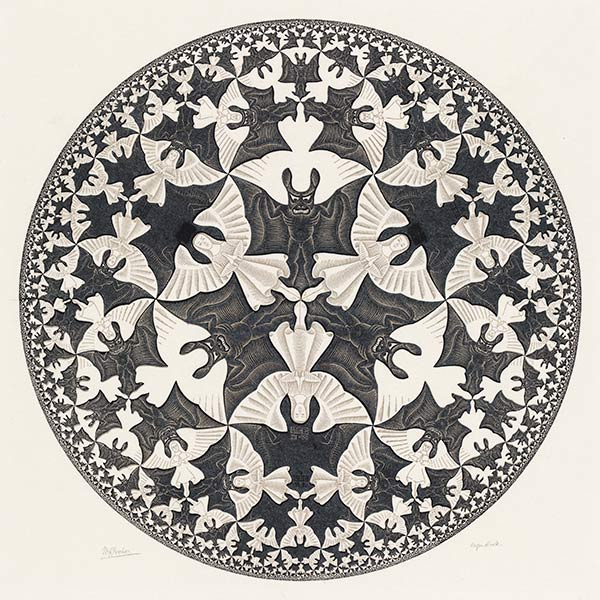
\includegraphics[scale=0.3]{img/circle-limit-IV-1960.eps}
 \captionsetup{labelformat=empty}
 \caption{埃舍尔《圆极限$\cdot$4》(又名天使与恶魔)1960}
 \label{fig:Penrose-triangle}
\end{wrapfigure}

不知在多久以前,我们的祖先仰望星空,面对浩瀚的星河,由衷地发出感叹,我们所在的世界究竟有多大?
作为智慧的生命,我们的思维超越自我,超越地球,超越宇宙,不断思考着无穷的概念。我们的祖先是从具体的事物中抽象出数了的概念。
例如狩猎得到的三头羊,采集得到三个果实,烧制了三个陶罐,进而得到抽象的数字三来代表任何三个东西。起初的数字大小有限,能够满足日常生活、狩猎、劳作。
随着文明的发展,我们开始进行贸易活动,出于记账的要求,所需要的数字逐渐变大。人们发展出种种计数系统,来掌握更大的数字。
终于,我们提出问题:最大的数是什么?对于这个问题,人们采用两种不同的态度。一种认为,这个问题没有意义,在古代,
掌握千百万这样的数已经足够生活中使用了。我们无需了解生活中用不上的大数。例如我们可以认为世界上沙子的数目是无穷的。
在古希腊,一万曾被认为是一个十分巨大的数,人们称它为murias,最终变成了myriad一词,意为“无数”\cite{De-linfini-2018}。无独有偶,佛教中也用“恒河沙数”来表达大到无法计算的数。在大乘佛教经典《金刚经》中,佛陀说:“以七宝满尔所恒河沙数三千大世界,以用布施。”另一种则不这么想,阿基米德,这位古希腊伟大的数学家认为,即使是充满全宇宙的沙子数目,也可以用一个数代表。在阿基米德在他的著作《数沙者》开篇中说:

“格朗王,有人认为沙子的数量是无穷的。我所说的沙子,并不单单地指叙拉古附近和西西里岛其余地方的沙子,还包括地球上所有角落能找到的沙子,无论那里有人还是无人居住。另一些人虽然承认沙子的数量并不是无穷大的,但他们认为,我们不可能写出一个足够大的数,使它在数量上超过地球上全部沙子所代表的数量。如果想象一个和地球体积同样大的沙体,而且要从地球上的大海和谷底算起,知道最高山峰的高度都填满沙子,这些人恐怕就更加肯定,世界上不可能有如此之大的数,可以用来表示堆积起这一巨大沙体所需要的沙子的数量。但是,我将向您证明,通过一系列几何张明——您之后也可以照着做——我命名了一些数字,写在我给宙克西珀的手稿中。其中一些数字不仅超过了以我刚刚描述过的方式填充地球所需要的沙子的数量,甚至超过了填充整个宇宙所需要的沙子数量。”

\begin{figure}[htbp]
%\begin{wrapfigure}{R}{0.4\textwidth}
 \centering
 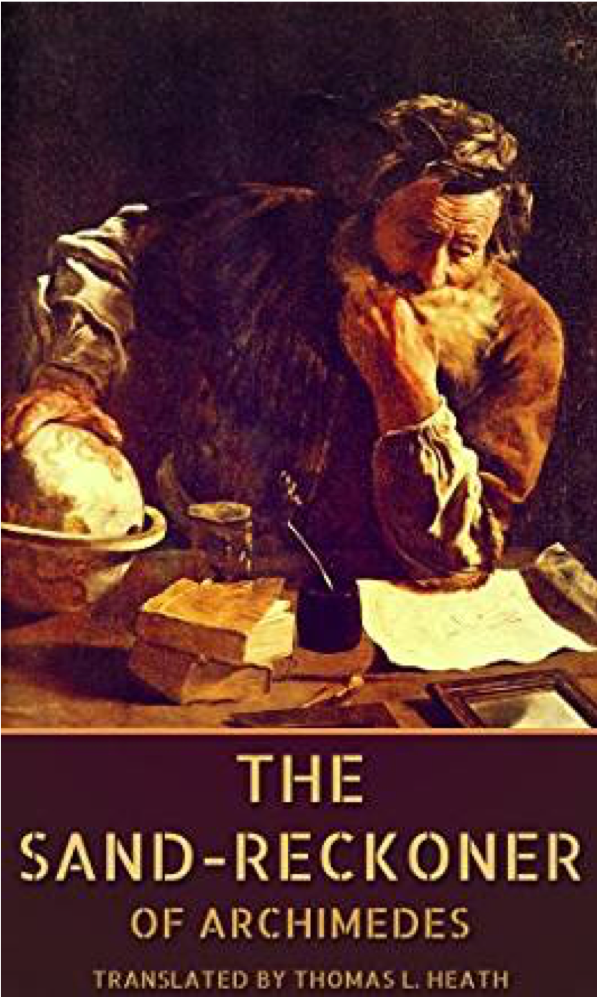
\includegraphics[scale=0.5]{img/Archimedes.eps}
 \captionsetup{labelformat=empty}
 \caption{《数沙者》,封面的阿基米德像是意大利画家多米尼克$\cdot$费蒂1620年创作的。}
 \label{fig:Archimedes}
%\end{wrapfigure}
\end{figure}

阿基米德认为填满宇宙“只”需要$10^{63}$粒沙子。这个宇宙的含义是指恒星天球,大约为两万倍地球的半径。今天我们知道可观测宇宙的尺寸大约为460亿光年,大约包含$3 \times 10^{74}$个原子\footnote{一说为$10^{80}$到$10^{87}$个基本粒子。}。在古希腊的时代,阿基米德的想法无疑是天才的,这几乎是无穷的具体化。我们从语言中,可以看到许多表达大数的单位的词语。例如下表是汉语中的大单位,从“兆”以后,每增加一万倍,就有一个对应的单位。(\cite{Noguchi2007},第31页)

\begin{center}
% for Pinyin tones: \={a}, \'{a}, \v{}, \.{a}
\begin{tabular}{|l|r|l|r|}
\hline
京            & $10^{16}$ & 载            & $10^{44}$ \\
\hline
垓(g\={a}i)   & $10^{20}$ & 极            & $10^{48}$ \\
\hline
秭(z\v{i})    & $10^{24}$ & \textbf{恒河沙}  & $10^{52}$ \\
\hline
穰(r\'{a}ng)  & $10^{28}$ & 阿僧祗(zh\={i})  & $10^{56}$ \\
\hline
沟            & $10^{32}$ & 那由他        & $10^{60}$ \\
\hline
涧            & $10^{36}$ & 不可思议      & $10^{64}$ \\
\hline
正            & $10^{40}$ & 无量大数      & $10^{68}$ \\
\hline
\end{tabular}
\end{center}

可以看到,汉语中这些大单位词汇,由许多来自佛教。包括恒河沙,它表示1后面跟着52个0。英语中的大单位如下表。从一开始,每增加一千倍就有一个对应的单位。这种万进位和千进位的不同,也是文化上的一种差异。

\begin{center}
\begin{tabular}{|l|r|l|r|l|r|}
\hline
thousand & $10^{3}$ & quattuordecillion & $10^{45}$ & octovigintillion & $10^{87}$ \\
\hline
million & $10^{6}$ & quindecillion & $10^{48}$ & novemvigintillion & $10^{90}$ \\
\hline
billion & $10^{9}$ & sexdecillion & $10^{51}$ & trigintillion & $10^{93}$ \\
\hline
trillion  & $10^{12}$ & septdecillion & $10^{54}$ & untrigintillion & $10^{96}$ \\
\hline
quadrillion  & $10^{15}$ & octodecillion & $10^{57}$ & duotrigintillion & $10^{99}$ \\
\hline
quintillion  & $10^{18}$ & novemdecillion & $10^{60}$ & \textbf{googol} & $10^{100}$ \\
\hline
sexillion    & $10^{21}$ & vigintillion & $10^{63}$ & & \\
\hline
septillion   & $10^{24}$ & unvigintillion & $10^{66}$ & & \\
\hline
octillion    & $10^{27}$ & duovigintillion & $10^{69}$ & & \\
\hline
noniliion  & $10^{30}$ & trevigintillion & $10^{72}$ & & \\
\hline
decillion  & $10^{33}$ & quattuorvigintillion & $10^{75}$ & & \\
\hline
undecillion   & $10^{36}$ & quinvigintillion & $10^{78}$ & & \\
\hline
duodecillion  & $10^{39}$ & sexvigintillion & $10^{81}$ & & \\
\hline
tredecillion  & $10^{42}$ & seprvigintillion & $10^{84}$ & & \\
\hline
\end{tabular}
\end{center}

表中最后一个大单位古格尔(googol)是在1920年由9岁的米尔顿$\cdot$西洛塔(Milton Sirotta)想出的名字。这个数字是1后面跟着100个零。著名的互联网公司谷歌的名字就来自它\cite{Wikipedia-Googol}。

\section{无穷概念的提出}

超越一切具体大数的无穷是否存在不仅是一个数学问题,还是一个哲学问题。无穷大还直接导致另一个概念——无穷小。古代中国的哲学家庄子在《天下篇》中说:“一尺之棰,日取其半,万世不竭。”,古希腊的哲学家,埃利亚学派的芝诺(Zeno of Elea)提出了著名的四个悖论,它们都与无穷有关。

\begin{figure}[htbp]
%\begin{wrapfigure}{R}{0.3\textwidth}
 \centering
 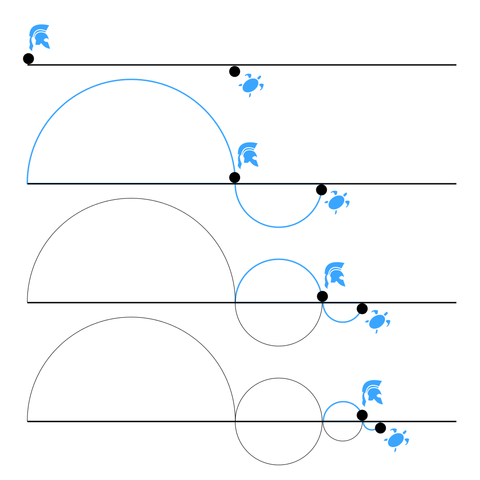
\includegraphics[scale=0.4]{img/Achilles-paradox.eps}
 %\captionsetup{labelformat=empty}
 \caption{阿基里斯与乌龟悖论}
 \label{fig:Achilles-paradox}
%\end{wrapfigure}
\end{figure}

第一个悖论最为人们所津津乐道。名叫阿基里斯与乌龟悖论。阿基里斯是荷马史诗《伊里亚特》中的英雄,以善跑著称。这个悖论说:如果让爬得很慢的乌龟在阿基里斯前面一段路程出发,那么阿基里斯将永远追不上乌龟。这时因为,阿基里斯为了赶上乌龟,必须先到达乌龟的出发点$A$,但当阿基里斯到达$A$点时,乌龟已经在这段时间前进到了$B$点。但当阿基里斯到达$B$点时,乌龟又已经到了前面的$C$点……以此类推,两者间的距离虽然越来越近,但阿基里斯永远落在乌龟的后面而追不上乌龟。如图\ref{fig:Achilles-paradox}所示。但是这与我们生活中的常识是不相符的。这个悖论的推理是如此让人信服,以至于千百年来吸引了无数学者的研究。刘易斯$\cdot$卡罗尔(Lewis Carrol)、侯世达(Douglas Hofstadter)甚至拿乌龟和阿基里斯作为文学作品中的主人公。

第二个悖论叫作“二分悖论”。这个悖论说,如果阿基里斯想从$A$到$B$,那么他必须先走到$1/2$的位置。同样在此之前,他必须要到达$1/4$的位置。而为了到达这一位置,他必须先到达$1/8$的位置……以此类推。由于这样的中点有无限多个,阿基里斯永远也也无法到达目的。芝诺的这个悖论实际上说明了运动根本无法发生。

\begin{figure}[htbp]
%\begin{wrapfigure}{R}{0.3\textwidth}
 \centering
 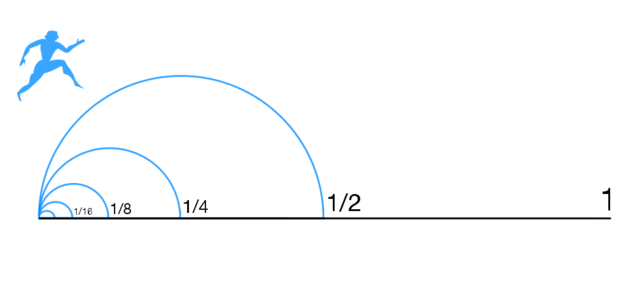
\includegraphics[scale=0.4]{img/Dichotomy-paradox.eps}
 %\captionsetup{labelformat=empty}
 \caption{二分悖论}
 \label{fig:Dichotomy-paradox}
%\end{wrapfigure}
\end{figure}

第三个悖论叫作“飞矢不动悖论”,它从另一个角度描述无穷导致运动无法发生。芝诺指出,任何物体待在相同的位置都不叫运动,可是飞行的箭矢在任一时刻不也是待在一个地方么?这样说来,自然飞失也是不动的。如果说前两个悖论是由于分割空间导致的,则这个悖论是由对时间的分割导致的。

\begin{figure}[htbp]
%\begin{wrapfigure}{R}{0.3\textwidth}
 \centering
 \subcaptionbox{飞失不动悖论}[0.3\linewidth]{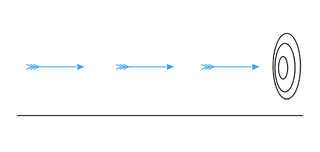
\includegraphics[scale=0.4]{img/Arrow-paradox.eps}} \\
 \subcaptionbox{运动场悖论}[0.7\linewidth]{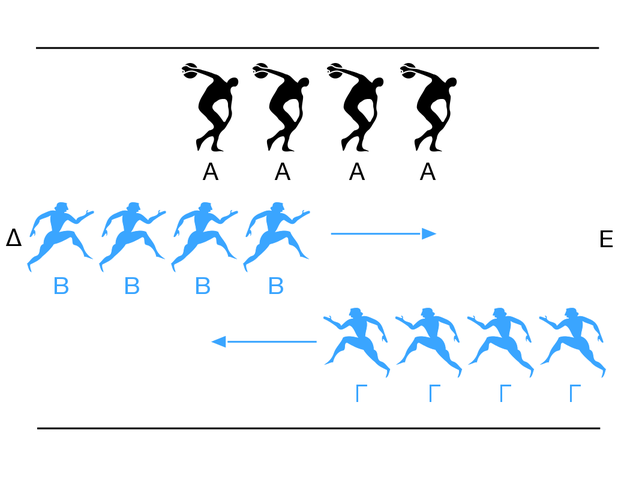
\includegraphics[scale=0.3]{img/Moving-rows-paradox.eps}}
 %\captionsetup{labelformat=empty}
 \caption{飞失不动和运动场悖论}
 \label{fig:Arrow-and-Moving-rows-paradox}
%\end{wrapfigure}
\end{figure}

第四个悖论叫作“运动场悖论”。这一悖论主要针对时间原子论的观点,即认为存在最小的不可分割的时间单位。如图\ref{fig:Arrow-and-Moving-rows-paradox}所示,运动场中有3列人。最初他们都收尾对齐。在最小的时间单元内,A列不动,B向右移一个单位,而$\Gamma$向左移动一个单位。容易得知,相对B而言,$\Gamma$其实移动列两个单位。这就意味着,应该存在这一让$\Gamma$相对于B移动一个单位的时间。而这一时间应该是最小单位时间的一半。但如果存在不可分割的“时间原子”,那么这两个时间就是相同的,即最小时间和它的一半相等。

\begin{wrapfigure}{L}{0.3\textwidth}
 \centering
 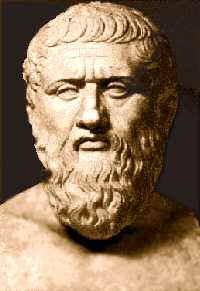
\includegraphics[scale=0.5]{img/Zeno.eps}
 \captionsetup{labelformat=empty}
 \caption{芝诺,约490BC - 425BC}
 \label{fig:Zeno-of-Elea}
\end{wrapfigure}

芝诺悖论并不复杂,稍加琢磨就能理解。但是导出的结果却出人意料。根据生活中的常识,运动和时间是如此真实,阿基里斯不可能赶不上乌龟。可是驳倒这些悖论却并不容易,从亚里士多德到罗素,从阿基米德到赫尔曼$\cdot$外尔,都对芝诺悖论提出了各种不同的解法\cite{Wikipedia-Zeno}。

芝诺(约公元前490年——公元前425年),古希腊哲学家,生于意大利半岛南部的埃利亚。所以我们常称其为埃利亚的芝诺(Zeno of Elea)。关于他的生平,缺少可靠的文字记载。据传,他早年是一个自学成才的乡村孩子,一生经历坎坷,最终遭到一位暴君的陷害而被拘捕、拷打、直至被处死\cite{HanXueTao16}。

芝诺是继毕达哥拉斯学派之后在意大利新出现的一个哲学学派——埃利亚学派的代表人物之一,这一学派的领袖是芝诺的老师巴门尼德。巴门尼德认为整个世界是个不变的整体,即“不变的一”,运动、变化与多样性都只是幻象。

芝诺以其悖论闻名。他一生曾巧妙地构想出40多个悖论,在流传下来的悖论中以关于运动的四个“无限微妙、无限深邃”的悖论最为著名。他提出这些悖论很可能是为他老师的哲学观点辩护。

芝诺悖论在当时曾给古希腊人造成深深的困惑。而芝诺悖论所涉及的对时间、空间、无限、连续、运动的看法,也都在极长的历史岁月中困扰着后来的哲学家和数学家。如何了解和认识无穷,如何使用无穷成为了摆在古希腊人面前必须解决的问题。

\subsection{无穷的哲学}
亚里士多德对芝诺悖论进行了深入的思考(我们今天对芝诺悖论的了解,其实是来自亚里士多德的著作《物理学》),并做出一项对后世数学发展具有深远影响的工作。他把无穷的概念区分为实无穷和潜无穷。所谓潜无穷或潜无限,是指无限在永远延伸着,是一种变化的、不断产生出来概念。它永远在构造中,永远完成不了,是潜在的,而不是实在的。自然数就是一种潜无穷,对于任何一个自然数,我们都可以找到它的后继,也就是一个更大的自然数。欧几里得几何中的直线也是一种潜无穷,我们可以按需延伸直线\footnote{欧几里得避免使用“无限延伸”这样的说法,而代之以按需任意延伸。这在古希腊是常见的一种处理。}。所谓实无穷是指把无限的整体本身作为一个实在的单位,是已经构造出来的东西。也就是把无限对象看作可完成的过程或无穷整体。

在做了这种区分后,亚里士多德承认存在潜无穷,但是拒绝承认实无穷的概念。他对实无穷的排斥深刻而长远地影响了日后数学的发展\cite{HanXueTao16}。亚里士多德代表了当时古希腊的哲学观点,关于潜无穷和实无穷的概念区分以及争论一直影响至今。尽管对无穷的概念仍然心存疑虑,古希腊的数学家们借助潜无穷的思想取得了令人赞叹的成就。其中之一就是欧几里得证明了存在无穷多的素数。这一证明被人们认为是历史上最优美的证明之一。

\begin{theorem}
《几何原本》第九卷,命题20。预先给定任意多的素数,则有比它们更多的素数\cite{Elements}。
\end{theorem}

欧几里得在叙述这个命题时,小心谨慎地避免使用无穷这样的说法,通观《几何原本》一书这样的例子还有很多。欧几里得在证明这个命题时,使用了著名的反证法。我们用现代的语言来描述这一证明。

\begin{proof}
假设只存在有限多个素数,$p_1, p_2, ..., p_n$。我们构造一个新数:
\[
p_1 p_2 ... p_n + 1
\]
也就是把这$n$个素数乘起来再加一。这个数要么是素数,要么不是素数。

\begin{itemize}
\item 如果它是素数,明显这个数不等于$p1$到$p_n$中的任何一个,这就在有限多个素数中又增加了一个新的素数;
\item 如果这个数不是素数,那么它就存在一个素因子$p$。但是由于$p1$到$p_n$中的任何一个都不能整除我们构造的这个数,所以素数$p$与任何$p_1$到$p_n$中的数都不同,是一个新的素数。
\end{itemize}
所以在任何情况下,我们都可以获得一个新的素数。这与有限个素数的假设矛盾,因此存在无穷多的素数。
\end{proof}

欧几里得用反正法得到了一种“存在性证明”,他证明了存在无穷多的素数,但却没有给出怎样得到这些素数。这在我们今天看来,是很自然的一种处理。然而在十九世纪末二十世纪初却引发了关于数学根本性的争论,我们将在下一章详细讲述这一内容。

\begin{wrapfigure}{L}{0.3\textwidth}
 \centering
 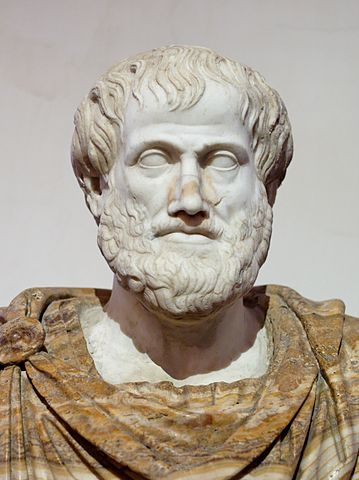
\includegraphics[scale=1]{img/Aristotle.eps}
 \captionsetup{labelformat=empty}
 \caption{亚里士多德,384BC - 322BC}
 \label{fig:Aristotle}
\end{wrapfigure}

亚里士多德是世界古代史上最伟大的哲学家、科学家和教育家之一,古希腊哲学的集大成者。他是柏拉图的学生,亚历山大大帝的老师。公元前384年,亚里士多德出生于希腊北部城市斯塔基拉(Stageira)。后人对他早年的生活所知甚少。17岁时,他赴雅典在柏拉图学园就读达20年,直到柏拉图去世后方才离开。这一时期的学习和生活对他一生产生了决定性的影响。苏格拉底是柏拉图的老师,亚里士多德又受教于柏拉图。在雅典的柏拉图学园中,亚里士多德表现的很出色,柏拉图称他是“学园之灵”。但亚里士多德可不是个只崇拜权威,在学术上唯唯诺诺而没有自己的想法的人。他努力的收集各种图书资料,勤奋钻研,甚至为自己建立了一个图书室。

公元前347年,柏拉图去世。两年后,亚里士多德离开了雅典——亚里士多德或许是带着失望的心情离开的,因为他并没有称为柏拉图思想的继承者。此后,他开始游历各地。公元前343年,亚里士多德被马其顿的国王腓力浦二世召唤回故乡,受国王的聘请,担任起当时年仅13岁的亚历山大大帝的老师。亚里士多德也运用了自己的影响力,对亚历山大大帝的思想形成起了重要的作用。正是在亚里士多德的影响下,亚历山大大帝始终对科学事业非常关心,对知识十分尊重。

公元前335年腓力浦去世,亚里士多德又回到雅典,并在那里建立了自己的学校。学园的名字叫做吕克昂(Lyceum)。在此期间,亚里士多德边讲课,边撰写了多部哲学著作。亚里士多德讲课时有一个习惯,边讲边漫步于走廊和花园,正是因为如此,学园的哲学被称为“逍遥派”或者是“漫步的哲学”。亚里士多德在这一期间也有很多著作,主要是关于自然学和物理方面的自然科学和哲学,而使用的语言也要比柏拉图的《对话录》晦涩许多。他的作品很多都是以讲课的笔记为基础,有些甚至是他学生的课堂笔记。因此有人将亚里士多德看作是西方的第一个教科书作者。

亚历山大去世后,雅典人开始奋起反对马其顿的统治。由于和亚历山大的关系,雅典人攻击亚里士多德,并判他为不敬神罪,当年苏格拉底就是因不敬神罪而被判处死刑的。但亚里士多德最终逃出了雅典。

公元前322年,亚里士多德因身染重病离开人世,终年六十三岁。

亚里士多德重视研究现实世界,他的精神财富正在于他的实证研究方法,这称为了现代科学的基本原则。此外,现在大学里面的院系划分方式,及其所反应的知识整理方式,也直接沿承自亚里士多德所提出的分类法。

\subsection{穷竭法与微积分}
与欧几里得的小心谨慎不同,古希腊的另一些数学家采用了较为实用的态度对待无穷,创造并发展了一种称为“穷竭法”的有力工具,取得了惊人的成就。

穷竭法由古希腊智人学派的代表人物安提丰(Antiphon,约前480——前410)首创。为了解决古希腊三大作图难题之一的圆化方问题\footnote{亦称为化圆为方问题,另外两个著名的难题是三分角问题和倍立方问题。任给一个圆,古希腊人希望找到只用尺规,能够作出同样面积的正方形。这个问题困扰了无数的数学家,直到19世纪后利用伽罗瓦的理论,才一举将它们题解决。三大难题被证明都是尺规不可解的。在英文中化圆为方square the circle被形容不可能做到的事情。},他提出用圆内接多边形逼近圆面积的方法来化圆为方。安提丰从一个圆内接正方形开始,不断将边数加倍得到正八边形、十六边形……不断重复这一过程,随着圆面积的逐渐“穷竭”,将得到一个边长越来越微小的圆内接正多边形。安提丰认为最终这一正多边形将与圆重合,这就是穷竭法的思想。后来古希腊伟大的数学家欧多克索斯对穷竭法进行了改进和严格化,使其成为解决面积、体积问题的一种有力的几何方法。为了理解这一方法,我们先要介绍著名的欧多克索斯——阿基米德公理,有时简称为阿基米德公理。

\begin{axiom}
\textbf{阿基米德公理(Axiom of Achimedes)}对于任意两个量$a$与$b$来说,总有自然数$n$使得$a \leq nb$。
\end{axiom}

阿基米德公理非常基本。在第二章中,我们介绍了欧几里得最大公约数算法,但是我们没有探讨这一算法是否能够结束。利用阿基米德公里就可以给出欧几里得算法一定能够结束的证明。利用这一基本原理,欧多克索斯指出:“给定两个不相等的量,如果从较大的量减去比它大一半的量,再从所余的量减去比这个余量大一半的量,重复这一过程,必有某个余量小于给定的较小的量。”这就是穷竭法背后的逻辑。

利用穷竭法,欧多克索斯证明了棱锥体积是同底同高棱柱体积的1/3,圆锥体积是同底同高圆柱体积的1/3。这些成果都记录在欧几里得的《几何原本》卷12中\cite{HanXueTao16}。

古希腊将穷竭法发展到最高成就的当属阿基米德,他取得了惊人的成就,计算出了圆周率$\pi$,证明圆面积公式,球体、锥体的表面积和体积公式,甚至找到了计算抛物线下面积的方法。被称为古希腊的数学之神。

%\begin{figure}[htbp]
\begin{wrapfigure}{R}{0.4\textwidth}
 \centering
 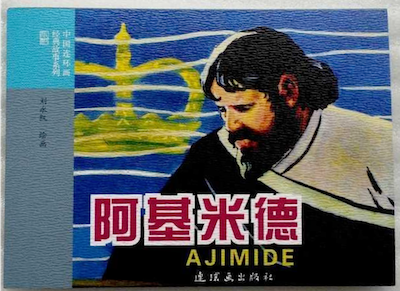
\includegraphics[scale=0.6]{img/Archimedes-book.eps}
 \captionsetup{labelformat=empty}
 \caption{小儿书《阿基米德》的封面}
 \label{fig:Archimedes-book}
\end{wrapfigure}
%\end{figure}

阿基米德(前287年——前212年),生于西西里岛的叙拉古王国。早年曾经在古希腊的学术中心亚历山大城跟随欧几里得学习。阿基米德后来回到了叙拉古,他的许多学术成果都是通过和亚历山大城的学者之间的往来信件保存下来的。虽然有关阿基米德的生平没有详细的记载,但是关于他的各种故事却广为流传、脍炙人口。

最著名的故事就是国王的王冠。叙拉古国王不知道他的王冠是否是纯金的,大臣们也一筹莫展,于是去请教阿基米德。阿基米德一直解不开这个难题,他废寝忘食,直到有一天洗澡的时候,看着浴缸里的水溢出来,突然得到了灵感。他从浴缸里一跃而出,光着身子跑到大街上,边跑边喊“尤里卡!尤里卡!”,这句希腊语Eureka的意思是“我找到了!”。阿基米德利用浮力和比重,最终发现王冠掺了假。他的这一发现就是每一个中学生都要学习的“阿基米德定律”。尤里卡后来被人们用来形容找到灵感的那一刹那。

TODO: 阿基米德发现球的体积是其外接圆柱体积的2/3。他觉得这一关系无比的美妙,因此决定死后在墓碑上刻下这一发现。
% Sphere: 4/3 pi r^3, Cylinder: pi r^2 * 2r = 2 pi r^3
% ==> S : C = 4/3 / 2 = 2/3

TODO:第二次不诺战争爆发了。面对敌人的围城,传说阿基米德设计了巨大的抛物面镜,把阳光汇聚到帆上烧毁了敌人的战船。阿基米德还设计了巨大的机械武器,可以瞬间击毁罗马战船。后来罗马军队攻陷了叙拉古城,一个罗马士兵冲进阿基米德的家里。阿基米德正在专注地在沙地上画着几何图形进行思考,他说出了那句著名的画:“你挡住了我的阳光。”感到被冒犯的罗马士兵挥刀杀死了面前的这个老人。古希腊最伟大的数学家就此停止了思考。

我们现在来看一下,阿基米德是如何利用穷竭法计算的圆周率。

TODO:如图\ref{fig:pi-exhaustion}所示,阿基米德在直径为1的圆内做一个内接多边形,同时在圆外做一个外切多边形。我们先看内接多边形的一条边和其上的圆弧,根据两点之间直线最短的几何公理,圆弧之长大于内接多边形的一条边长,故而圆的周长大于内接多边形的周长。同样可以得知,圆的周长小于外切多边形的周长。由于直径为1的圆,其周长恰好就是圆周率。这样我们就可以得到关系式:

\[
  C_o < \pi < C_i
\]

\begin{figure}[htbp]
%\begin{wrapfigure}{R}{0.4\textwidth}
 \centering
 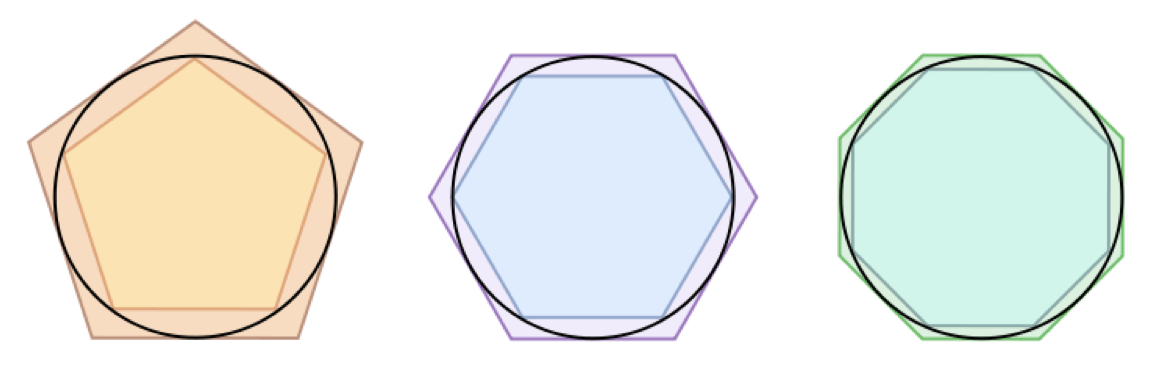
\includegraphics[scale=0.5]{img/pi-exhaustion.eps}
 %\captionsetup{labelformat=empty}
 \caption{用穷竭法计算圆周率}
 \label{fig:pi-exhaustion}
%\end{wrapfigure}
\end{figure}

其中$C_o$、$C_i$分别外外切多边形和内接多边形的周长。不断加大边数,就可以越来越精确地获得$\pi$的范围。阿基米德将边数驾到到256,得出圆周率在3.1415和3.1416之间。这一记录直到南北朝时,才由我国的数学家祖冲之打破。

穷竭法的缺点是,它仍然是基于古希腊几何的一种方法,使用起来非常复杂。这部分是由于古希腊人不接受无理数,于是把几何量和“数”的概念隔离开。另一方面,古希腊整体上试图避免使用无穷大和无穷小的概念。

另一位使用穷竭法的大师是天文学家托勒密。他首次为天体运行建立了模型,地球位于宇宙的中心,月球,太阳,和其他行星则在嵌套在一起的球面上运行,最外层则是恒星天球。

亚历山大时代之后,古希腊文明的数学成果遭受了巨大的打击。罗马人征服后,迪奥多西(Theodosius)废除了异教,并且392年下令拆毁古希腊人的神庙。成千上万的希腊图书被罗马人焚毁,在公元前47年。罗马人纵火焚烧亚历山大港口内的船只,火势蔓延烧毁了藏书最丰富的古代图书馆。保存大量希腊著作的塞拉皮斯神庙也被摧毁,写在羊皮上的著作被刮掉而改写宗教著作。

对希腊文明的最后打击是公元640年新崛起的阿拉伯帝国对埃及的征服。残剩的图书被焚毁殆尽。征服者奥马尔说:“这些书的内容或许我们也有,那么我们不必读它;这些书里或许有反对我们的内容,那我们不准读它。”因此亚历山大城的浴室里接连有6个月用羊皮纸来烧水\cite{M-Kline-2007}。

每次读到此处的历史,不仅让人痛心疾首,唏嘘不已。焚书的悲剧在南美洲,在秦帝国,自古及今不断上演。埃及被占领后,一些学者迁居到东罗马帝国的首都君士坦丁堡。阿拉伯帝国后来也把一部分古希腊的数学著作翻译成阿拉伯文。巴格达的智慧宫成为了当时世界学术的中心。中世纪后,欧洲的学者又逐渐把这些阿拉伯文的著作再次译成拉丁文。伴随着文艺复兴,也是数学和哲学的复兴。接过阿基米德和穷竭法的接力棒的是德国天文学家约翰内斯$\cdot$开普勒。托勒密的宇宙模型无法解释行星反向运动的现象,通过分析行星的观测数据,哥白尼提出了日心说,从托勒密模型需要的X个圆简化到了Y个圆。但仍然和观测有一些偏差。开普勒潜心分析德国天文学家第谷的数据Z年,终于破解了行星运动的规律,这就是我们今天熟知的开普勒三大行星运动定律。按照开普勒定律,行星的运行轨迹并不是圆,而是一个椭圆,太阳在椭圆的一个焦点上。行星在单位时间内扫过的面积相同,因而在椭圆上有时速度快(例如在近日点附近),有时速度慢(例如在远日点附近)。分析这样复杂的数学模型需要新的工具,古希腊的穷竭法太过复杂笨重。开普勒于是进行了简化,他甚至还用自己简化的方法计算出了葡萄酒桶的容积。

接下来迈出重要一步的是笛卡尔和费马。通过解析几何,人们终于将数和几何结合了起来,并且在莱布尼茨和牛顿的手中发展出了微积分。微积分中的一个绕不开的概念是无限小量。并且在积分中必然要涉及无限多个量的累加。值得一题的是1665年,对微积分的发展做出重要贡献的学者约翰$\cdot$沃利斯首次引入了现代的无穷符号$\infty$。

尽管微积分的基础尚有很多争论,这一代表西方现代精神的风帆在18世纪乘风破浪。这是一个英雄辈出的时代,伯努利家族、欧拉、拉格朗日奔放地使用着微积分和无穷级数,解决了一个又一个以前无法想象的难题,在天文学,力学、流体力学上开拓进取。

\section{潜无穷与编程}
对微积分基础的严密化直接导致了人们对实无穷的思考与激烈争论。在此之前,我们先来看一下在编程中,无穷是如何被体现的。计算机使用的是有限的资源,历史上,整数在机器内部表示为二进制形式。因为只用有限的二进制位,所以能表示的范围是有限的。$m$位二进制最大可以表示$2^m-1$的整数,它的二进制形式为11...1,即$m$个1。例如16位整数的最大值是$2^{16}-1 = 65535$。由于这个原因,如果多个元素集合的基数用整数表示,则元素的数目也是有限的。在传统的编程中,通常使用数组来容纳多个元素,为了节省内存通常要求事先确定数组大小的上限,例如下面的C语言程序定义了一个容量为10个元素的整数数组:

\begin{verbatim}
int a[10];
\end{verbatim}

这里涉及两个概念,一个是序数,一个是基数。简单来说,序数就是我们在数数时赋予对象的一个标签。而基数是一个集合中元素的个数。早期的编程中,基数和序数都是有限的。这显然无法直接表达无穷的概念。在计算机科学发展的初期,这是完全可以理解的。那时的设备非常昂贵。人们根本不会想到使用无穷来直接解决具体的问题。然而随着时代的发展,成本逐渐降低,人们不再满足在解决问题之前,预先预测出所需集合的大小。于是在一些编程环境中,开始支持动态增长的数组。人们称之为容器或者向量,可以随时按照需要向其中增加元素。现实中,即使是动态容器,其中的元素个数仍然是有限的,不能超过表示的上限。为此人们又发展出了链表结构。如本书第一章中介绍的那样,每个元素用一个节点代表,一个接一个链接起来,最后一个元素指向一个特殊的空节点表示结尾。这样我们无须知道整条链表的基数,却能从表头开始,逐一前进到表中任何位置。只要存储空间允许,链表可以任意长。这样就创造了表达潜无穷的可能。

可是链表和潜无穷终究还差了一步。我们认为自然数是无限延伸着的潜无穷,如果用链表表示自然数,不管链表有多长,例如$n$,我们必须把0到$n$这些数都逐一填入其中。但这只表示了序列0, 1, ..., $n$,而不是自然数序列0, 1, ..., $n$, ...

为此,人们提出了惰性求值的概念。所谓惰性求值,就是并不立即计算一个变量的值,而是把计算推迟到需要这个值的时候。具体到自然数的例子,根据第一章介绍的皮亚诺公理,任给一个自然数$n$,都存在它的后继$n+1$。而第一个自然数是0。这样自然数就可以表示为:

\[
N = iterate(n \mapsto n + 1, 0)
\]

其中$iterate$的定义为:

\[
iterate(f, x) = x : iterate(f, f(x))
\]

我们来看一下自然数产生的头几步,简单期间,我们命名$succ(n) = n \mapsto n +1$

\[
\begin{array}{rcll}
iterate(succ, 0) & = & 0 : iterate(succ, succ(0)) & iterate\text{的定义}\\
                 & = & 0 : iterate(succ, 1) & succ(0) = 0 + 1 = 1 \\
                 & = & 0 : 1 : iterate(succ, succ(1)) & \\
                 & = & 0 : 1 : iterate(succ, 2) & \\
                 & = & 0 : 1 : 2 : iterate(succ, 3) & \\
                 & = & ... & \\
\end{array}
\]

如果没有惰性求值,上述过程就一会一直计算下去,永不终止。这是无法用来解决实际问题的。为此我们必须把链表的链接操作实现为惰性的,其中一种方法就是利用第二章介绍的$\lambda$表达式:

\[
x : xs = cons(x, () \mapsto xs)
\]

这种表达式$() \mapsto exp$通常叫作$delay(exp)$,它产生一个不带有参数函数,对这个函数求值得到结果$exp$。

\begin{figure}[htbp]
%\begin{wrapfigure}{R}{0.4\textwidth}
 \centering
 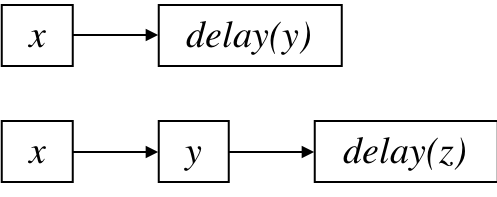
\includegraphics[scale=0.5]{img/stream-cons.eps}
 %\captionsetup{labelformat=empty}
 \caption{链表指向的下一个节点是一个$lambda$表达式,强制求值后产生一个新节点}
 \label{fig:stream-cons}
%\end{wrapfigure}
\end{figure}

这样,当把$x$和$xs$链接到一起的时候,我们并不会求出$xs$的值,而是把它放入一个$\lambda$表达式中,推迟到将来再求值。这样改动后,产生自然数时就变成:

\[
\begin{array}{rcll}
iterate(succ, 0) & = & 0 : iterate(succ, succ(0)) & iterate\text{的定义}\\
                 & = & cons(0, () \mapsto iterate(succ, succ(0))) & \text{惰性链接} \\
\end{array}
\]

计算到此为止,而不会继续进行下去。结果是一个列表,表中第一个元素是0,下一个元素是一个$\lambda$表达式。如果想求出后继的元素,我们必须强制让列表求值。

\[
next(cons(x, e)) = e()
\]

这样,将$next$应用到$cons(0, () \mapsto iterate(succ, succ(0)))$就得到:

\[
\begin{array}{cll}
  & next(cons(0, () \mapsto iterate(succ, succ(0)))) & \\
= & iterate(succ, succ(0)) & next\text{的定义} \\
= & iterate(succ, 1) & succ\text{的定义} \\
= & 1 : iterate(succ, succ(1)) & iterate\text{的定义} \\
= & cons(1, () \mapsto iterate(succ, succ(1))) & \text{惰性链接}
\end{array}
\]

计算到这里又停了下来。不断对$N$计算$next$,就源源不断的获得了一个一个的自然数。人们称这种模型为“流”(Stream),用它来表示潜无穷。我们甚至可以定义一个函数从潜无穷的流中取得前$m$个自然数。

\[
\begin{array}{l}
take\ 0\ \_\ = [] \\
take\ n\ cons(x, e)\ = cons(x, take(n-1, e())) \\
\end{array}
\]

例如$take\ 8\ N = [0, 1, 2, 3, 4, 5, 6, 7]$。本章附录给出了几种语言中,用流的方法定义自然数潜无穷的一些例子。

\begin{Exercise}
\Question{第一章中,我们用叠加操作实现了斐波那契数列,如何用$iterate$定义斐波那契数列潜无穷?}
\Question{用叠加操作定义$iterate$。}
\end{Exercise}

\section{实无穷的思考}
亚里士多德的影响是深远的。在两千多年的时间里,数学家和哲学家们不断思考无穷的本质,大多数人能够接受潜无穷的观念。但是对于实无穷,却产生了严重的分歧。在很长一段时间,人们认为实无穷就是无所不能的上帝,或者只有上帝才能掌握实无穷。一些对实无穷的尝试带来的是令人困惑的矛盾结果。例如,假设全体自然数是一个实无穷。由于自然数从头开始,间隔着一个偶数一个奇数,人们自然认为全体偶数是全体自然数的一半。可是任何自然数乘以2,就得到了一个偶数,反之,任何偶数除以2,也对应这个一个自然数。这样看来全体自然数和全体偶数存在一一对应关系。于是这两个实无穷是同样多的。究竟是自然数多还是偶数多呢?

%\begin{figure}[htbp]
\begin{wrapfigure}{L}{0.4\textwidth}
 \centering
 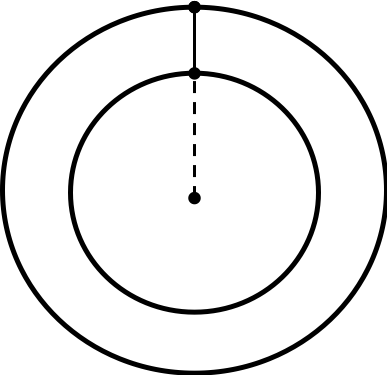
\includegraphics[scale=0.5]{img/circles-paradox.eps}
 %\captionsetup{labelformat=empty}
 \caption{同心大圆上任意一点都可通过半径对应到小圆上的唯一点}
 \label{fig:circles-paradox}
\end{wrapfigure}
%\end{figure}

现代科学之父伽利略在1636年的著作《论两种新科学及其数学演化》中提出一个类似的悖论。如果将每个自然数平方,得到的新序列1, 4, 9, 16, 25, ...和自然数存在一一对应关系。这样看来完全平方数和自然数一样多。可是常识却告诉我们,平方数很稀疏,自然数要比平方数多得多。这一矛盾通常称为“伽利略悖论”。

不仅在算数上,在几何上人们同样发现了类似的悖论。人们注意到每条半径都把两个同心圆上的点连接起来。大圆上任意一点都一一对应到小圆上的一点。这样看来两个圆上的点同样多,可是常识通常认为大圆上的点更多。

由于这些悖论的出现,人们接受了亚里士多德的观点,采取的回避的态度。伽利略发现无法解释自然数和平方数孰多孰少后说:因此我们不能说自然数构成一个集合。人们拒绝“全体自然数”这类说法,否认实无限的存在。

%\begin{figure}[htbp]
\begin{wrapfigure}{R}{0.4\textwidth}
 \centering
 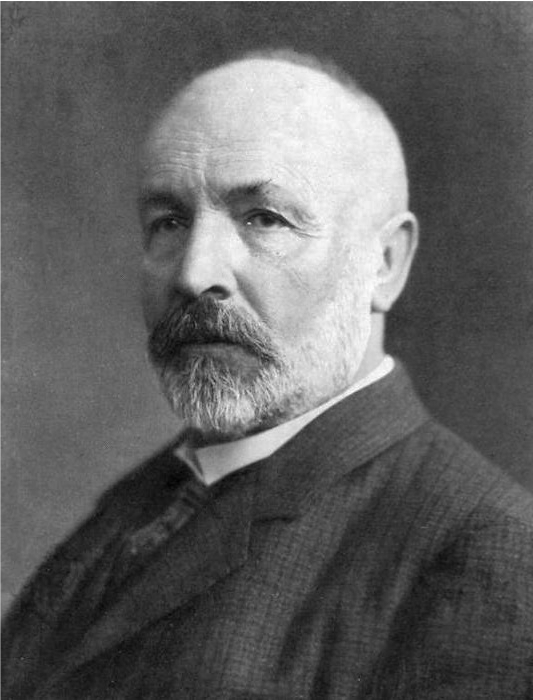
\includegraphics[scale=0.5]{img/Cantor.eps}
 \captionsetup{labelformat=empty}
 \caption{格奥尔格$\cdot$康托尔(1845-1918)}
 \label{fig:Cantor}
\end{wrapfigure}
%\end{figure}

终于,在伽利略身后两百年,德国数学家康托尔带领人们闯入了无穷王国。康托尔重新思考了陷入矛盾的一系列悖论,看起来问题的关键在于人们的常识——即整体一定大于部分。这一定是对的么?近代科学的发展一再告诉我们,人们根深蒂固用于具体事物的常识有时并不适用于更加抽象的概念。相对论挑战着人们的时空观常识——我们的所在的空间并不一定是熟悉的欧几里得空间,量子力学力学挑战着人们的因果观常识——随机性主导着量子世界。常识一旦突破,就会打开一片从未见过的新天地,从而带来巨大的认知进步。康托尔大胆地思考,如果我们接受“部分能够等于整体”的观点,通向无穷的大门就打开了。他提出“可以通过一一对应的方法来比较两个集合的大小,实无限是确实存在的概念。”

为了比较两个集合的大小,康托尔定义:如果能够建立集合$M$和集合$N$中元素的一一对应关系,那么这两个集合具有相同的基数(cardinal number),或者说它们是“等势”的\footnote{可以回想第三章中我们介绍的“同构”概念。}。对于有限集,显然这一结论是正确的,推广到无限集,根据这一定义,全体偶数和全体自然数一样多!完全平方数和自然数一样多,小圆上的点和大圆上的点也是一样多……甚至康托尔的挚友戴徳金干脆这样定义无穷集合:如果一个集合的部分和整体可以具有相同的基数,那么这个集合是无穷集合。

\subsection{无穷王国的花园}

让我们来欣赏一下康托尔为我们打开的无穷王国中的花园。数学家希尔伯特为了帮助人们理解康托尔的无穷集合概念,在1924年的国际数学家大会上,讲了这样的一个故事。

有一个神奇的旅馆,拥有无穷多的房间。在旅游旺季的时候,旅馆住满了客人,已经满员了。这一天晚上,又来了一名客人。要是一般的旅馆,就只能拒绝这个新客人入住,让他另找一家了。旅店经理希尔伯特说:“没问题,住得下。”他于是指挥客人,让1号房间的客人搬到2号房间去,2号房间的客人搬到3号房间去,3号房间的客人搬到4号房间去……每个房间的客人都搬到下一个房间去。这样就空出了1号房间给新来的这位客人。

故事没有结束。第二天,旅店迎来了一个神奇的旅游团,不同于普通的旅游团,它有无穷多个游客。酒店经理希尔伯特又说:“没问题,住得下。”他指挥房间里的客人。让昨天住进1号房间的那位新客人搬到2号房间去,让2号房间的客人搬到4号房间去,让3号房间的客人搬到6号房间去……每个房间的客人都搬到房间号2倍的那个房间去。由于酒店又无穷多的房间,所以这样一搬,2, 4, 6, ...这些偶数房间住着原来的客人。而1, 3, 5, ...这些奇数房间空出来,有无穷多间。刚好可以让旅游团的人一人一间住下。

故事更加曲折了。到了第三天,旅馆门前车水马龙,来了无穷多的神奇旅游团,每个旅游团都有无穷多个游客。希尔伯特的无穷旅馆还能住下么?在揭晓答案之前,我们先回顾一下前两天的故事。

\begin{figure}[htbp]
%\begin{wrapfigure}{R}{0.4\textwidth}
 \centering
 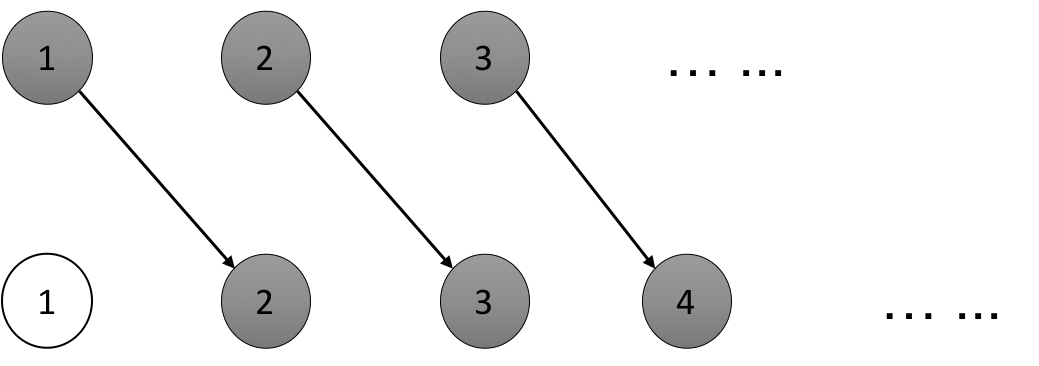
\includegraphics[scale=0.4]{img/Hilbert-hotel-1.eps}
 %\captionsetup{labelformat=empty}
 \caption{希尔伯特无穷旅馆的第一天}
 \label{fig:Hilbert-hotel-1}
%\end{wrapfigure}
\end{figure}

如图\ref{fig:Hilbert-hotel-1}所示,在第一天的故事中,我们让每个客人搬到下一个房间去,从而空出1号房间。实际上,这建立了图中上下两行灰色圆形之间的一种对应关系$n \leftrightarrow n+1$。这告诉我们一个有趣的事实,无穷加上1还是无穷。不仅如此,即使来了有限多名$k$位新客人,我们可以重复这一“腾笼换鸟”的过程$k$次,仍然能够让满员的宾馆住下他们。这相当于:

\bean
\infty + 1 = \infty \\
\infty + k = \infty \\
\eean

\begin{figure}[htbp]
%\begin{wrapfigure}{R}{0.4\textwidth}
 \centering
 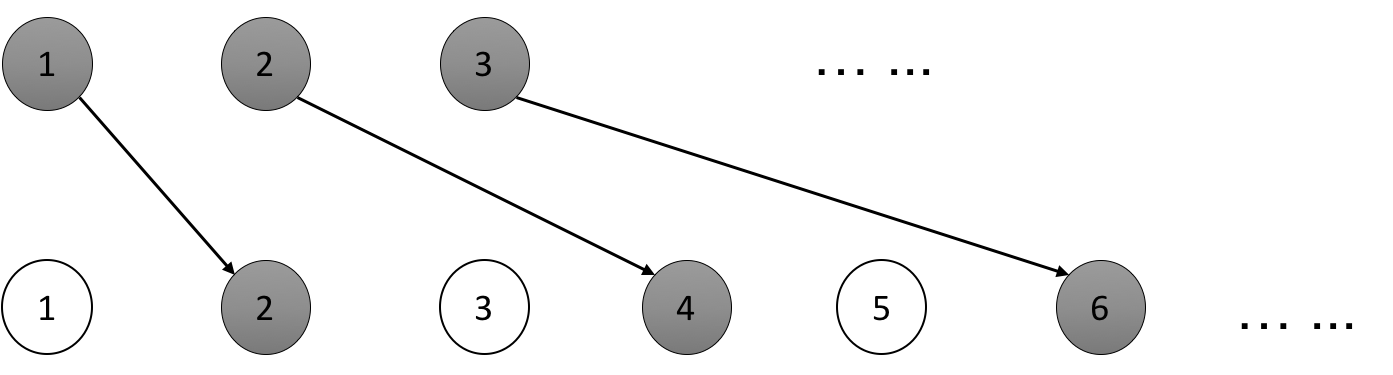
\includegraphics[scale=0.4]{img/Hilbert-hotel-2.eps}
 %\captionsetup{labelformat=empty}
 \caption{希尔伯特无穷旅馆的第二天}
 \label{fig:Hilbert-hotel-2}
%\end{wrapfigure}
\end{figure}

第二天的故事如图\ref{fig:Hilbert-hotel-2}所示,我们实际上建立了自然数到偶数间的一一映射,从而空出了无穷多间奇数房间,而这些空房间又和旅游图的无穷多位客人之间建立了一一映射,这恰好是奇数到自然数间的一一映射。第二天的故事告诉我们,无穷加上无穷仍然是无穷。

\[
\infty + \infty = \infty
\]

尽管符号相同,我们还是不禁会问,等号左边的无穷和等号右边的无穷是相同的么?无穷之间还能再比较大小么?我们稍后会看到,正是这个问题,导致了康托尔的进一步研究。在希尔伯特旅馆的问题中,这些无穷之间都可以建立一一对应关系,因此它们是“相等”的。我们把和自然数一一对应的无穷叫作可数无穷。

\begin{figure}[htbp]
\centering
\begin{tikzpicture}
  \draw[step=1, very thin, gray] (0, 0) grid (5, 5);
  \draw[->] (-0.25, 0) -- (6, 0) coordinate (x axis);
  \draw[->] (0, -0.25) -- (0, 6) coordinate (y axis);
  \foreach \x in {0, 1, 2, 3, 4, 5}
    \path (\x, -0.25) node[left] {\x};
  \foreach \y in {1, 2, 3, 4, 5}
    \path (-0.25, \y) node[below] {\y};
  \foreach \i / \x / \y in {0/0/0, 1/1/0, 2/0/1, 3/0/2, 4/1/1, 5/2/0, 6/3/0, 7/2/1, 8/1/2, 9/0/3, 10/0/4}{
    \path (\x, \y) coordinate (N\i);
    \fill (N\i) circle (1pt) node[above right=3pt of N\i] {\i};
  }
  \foreach \i in {0,...,9} {
    \pgfmathsetmacro{\j}{\i+1}
    \draw[-latex, thick] (N\i) to (N\j);
  }
\end{tikzpicture}
\caption{对无穷个无穷的一种编号方案}
\label{fig:NNtoN}
\end{figure}

要想解决希尔伯特旅馆第三天的问题,我们需要思考能否在无穷个无穷旅游团和无穷个房间之间建立一一对应。有人说,可以先让第一个旅游团依次入住1, 2, ...号房间,然后让第二个旅游团的第一个客人住在$\infty + 1$号房间,第二个客人住$\infty + 2$号房间……以此类推。但是这样的思路是行不通的,我们事先并不知道究竟是房间多,还是客人多。考虑安排客人的过程,第二个旅游团的第一个客人永远不知道第一个旅游团何时入住完,从而确定自己应该搬入的房间。与之相反,在第一天的故事中,一旦1号房间的客人搬入2号房间,新客人就可以立即入住了。尽管每个客人都依次搬入下一个房间是一个无穷无尽的过程。第二天的故事中也是如此,原1号房间的客人搬到2号房间的同时,旅游团中的第1个客人就可以搬入空出来的1号房间了,接下来原2号房间的客人搬到4号房间,原3号房间的客人搬到6号房间,此时旅游团中的第2个客人就可以搬入3号房间了……

图\ref{fig:NNtoN}给出了一种编号方案。为了方便,我们让每个旅游团的第一个客人编号为0,第二个客人编号为1,第三个客人编号为2……,我们把已经在旅馆中入住的客人编号为0号旅游团,新来的第一个旅游团编号为1号团,第二个旅游团编号为2号团……在这个图中,每个客人就对应无穷伸展的方格子中的一个点。同样我们让旅馆的房间号也从0开始。

现在我们按照这个顺序安排入住:第0号团的第0号客人入住0号房间,第0号团的第1号客人入住1号房间,第1号团的第0号客人入住第2号房间,第2号团的第0号客人入住3号房间,第1号团的第1号客人入住4号房间……这样按照图中往返画“之”字形,就可以逐一、并且毫无遗漏地安排每个客人入住。我们在无穷个旅游团的每个客人和无穷个房间之间建立了一一映射。希尔伯特的旅馆神奇地容纳了“二维”的无穷。

\begin{Exercise}
\Question{我们用图\ref{fig:NNtoN}建立了房间和任意旅游团的客人间的一一映射。第$i$号旅游团的第$j$号客人应该入住几号房间?第$k$个房间里住了哪号旅游团的哪位客人?}
\Question{希尔伯特旅馆第三天的故事的解法并不唯一,图\ref{fig:PWW-NNtoN}是《无需语言的证明》一书的封面。你能根据此图给出另一种编号方案么?
\begin{figure}[htbp]
 \centering
 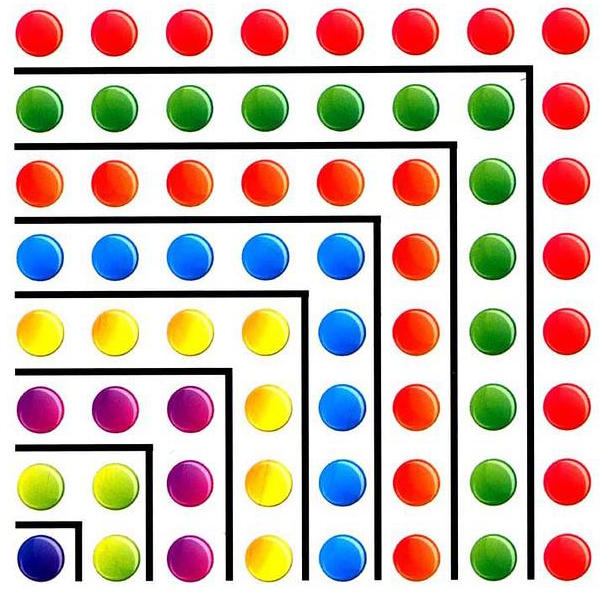
\includegraphics[scale=0.2]{img/PWW.eps}
 \caption{《无需语言的证明》封面局部}
 \label{fig:PWW-NNtoN}
\end{figure}
}
\end{Exercise}


\subsection{一一对应与无穷集合}

\begin{figure}[htbp]
%\begin{wrapfigure}{R}{0.4\textwidth}
 \centering
 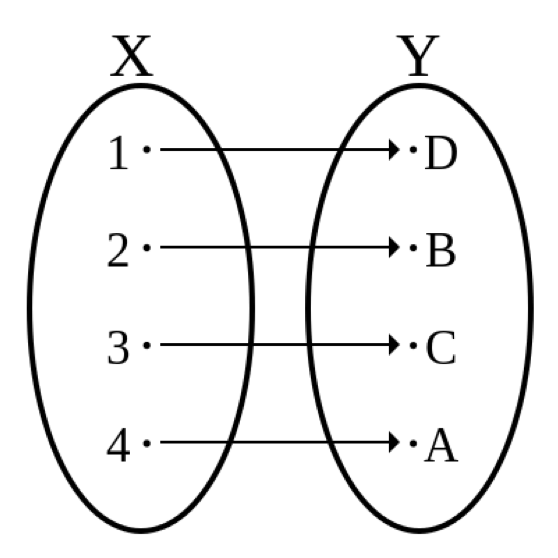
\includegraphics[scale=0.4]{img/bijection.eps}
 %\captionsetup{labelformat=empty}
 \caption{集合间的一一对应}
 \label{fig:bijection}
%\end{wrapfigure}
\end{figure}

康托尔与戴得金

利用(可数)无穷定义斐波那契数列和哈明数列

有些编程环境,所有的求值默认都是惰性的,在这样的环境中,我们甚至可以直接拿潜无穷流进行复杂的计算。例如下面是另一种自然数的定义方法:

\[
N = 0 : map(succ, N)
\]

它的含义是,$N$是一个潜无穷,代表自然数。第一个自然数是0,从第二个自然数开始,后面每个自然数,都等于前一个自然数的后继。如同下面的表格:

\begin{tabular}{|r|r|l|l|l|l|}
\hline
                 & $N$: & 0 & 1 & 2 & ... \\
\hline
                 & $map(succ, N)$: & $succ(0)$ & $succ(1)$ & $succ(2)$ & ... \\
\hline
$0 : map(succ, N)$: & 0 & 1 & 2 & 3 & ... \\
\hline
\end{tabular}

TODO: Fibonacci sequence.

流的范畴论解释

\subsection{可数无穷与不可数无穷}
可数无穷和不可数无穷——实数集

对角线证明

\subsection{戴得金分割}
戴得金分割

连续统假设

\section{无穷与艺术}
无穷与艺术

非欧几何(无穷与无界)

%\begin{wrapfigure}{L}{0.4\textwidth}
\begin{figure}[htbp]
 \centering
 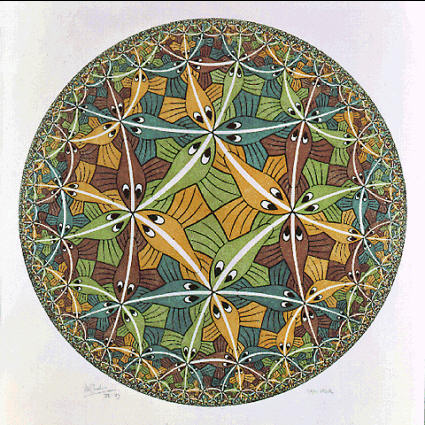
\includegraphics[scale=1.0]{img/circle-limit-III-1959.eps}
 \captionsetup{labelformat=empty}
 \caption{埃舍尔《圆极限$\cdot$3》1959}
 \label{fig:Penrose-triangle}
\end{figure}
%\end{wrapfigure}

\section{附录:例子代码}

使用流定义自然数潜无穷,然后从中取出前15个自然数。Java语言1.8中的例子:

\lstset{frame=single, language=Java}
\begin{lstlisting}
IntStream.iterate(1, i -> i + 1);

IntStream.iterate(1, i -> i + 1)
        .limit(15).forEach(System.out::println);
\end{lstlisting}

Python语言版本3中的例子:

\lstset{frame=single, language=Python}
\begin{lstlisting}
def naturals():
    yield 0
    for n in naturals():
        yield n + 1
\end{lstlisting}

Haskell语言的例子:

\lstset{frame=single, language=Haskell}
\begin{lstlisting}
nat = [1..]

take 15 nat
\end{lstlisting}

Haskell语言中使用递归定义自然数潜无穷:

\lstset{frame=single, language=Haskell}
\begin{lstlisting}
nat = 1 : (map (+1) nat)

take 15 nat
\end{lstlisting}

Haskell语言中使用递归定义斐波那契数列潜无穷。获取前15个斐波那契数,以及计算第1500个斐波那契数。

\lstset{frame=single, language=Haskell}
\begin{lstlisting}
fib = 0 : 1 : zipWith (+) fib (tail fib)

take 15 $ fib
[0,1,1,2,3,5,8,13,21,34,55,89,144,233,377]

fib !! 1500
13551125668563101951636936867148408377786010712418497242133543153221487310
87352875061225935403571726530037377881434732025769925708235655004534991410
29242495959974839822286992875272419318113250950996424476212422002092544399
20196960465321438498305345893378932585393381539093549479296194800838145996
187122583354898000
\end{lstlisting}

% Mathematicians aren't satisfied because they know there are no solutions up to four million or four billion, they really want to know that there are no solutions up to infinity. -- Andrew Wiles



\ifx\wholebook\relax \else
\begin{thebibliography}{99}

\bibitem{De-linfini-2018}
[法] 让-皮埃尔$\cdot$卢米涅,马克$\cdot$拉雪茨-雷 著,孙展 译. 从无穷开始——科学的困惑与疆界. 人民邮电出版社. 2018. ISBN: 9787115479198

\bibitem{Noguchi2007}
[日] 野口哲也 著,刘慧 韩丽红 译. 数学原来可以这样学. 湖南人民出版社. 2014. ISBN: 9787556100897
% Tetsunori Noguchi. SUGAKUTEKI SENSE GA MINITUKU RENSHUCHO.

\bibitem{Wikipedia-Googol}
Wikipedia. ``Googol''. \url{https://en.wikipedia.org/wiki/Googol}

\bibitem{Wikipedia-Zeno}
Wikipedia. ``Zeno's Paradoxes''. \url{https://en.wikipedia.org/wiki/Zeno's_paradoxes}

\bibitem{HanXueTao16}
韩雪涛 ``数学悖论与三次数学危机''. 人民邮电出版社. 2016, ISBN: 9787115430434

\bibitem{Elements}
[古希腊] 欧几里得 著,兰纪正 朱恩宽 译,梁宗巨 张毓新 徐伯谦 校订 ``几何原本''. 译林出版社. 2014, ISBN: 9787544750066

\bibitem{M-Kline-2007}
[美] M$\cdot$克莱因 著 李宏魁 译 ``数学:确定性的丧失'' 湖南科学技术出版社,2007年4月 ISBN: 978-7-5357-1857-0
% Morris Kline ``Mathematics: The Loss of Certainty''. Oxford University Press, 1980.

\end{thebibliography}

\expandafter\enddocument
%\end{document}

\fi
